% Created 2024-11-12 Tue 12:19
% Intended LaTeX compiler: pdflatex
\documentclass[10pt]{article}
% =================================BASE====================================%
\usepackage[left=2cm,right=2cm,top=2cm,bottom=2cm]{geometry} % Marges
\usepackage[T1]{fontenc} % Nécessaire avec FrenchBabel
\usepackage[utf8]{inputenc} % Important pour symboles Francophones, é,à,etc
\usepackage{csquotes} % Recommandé par PDFLatex lors de la compilation. 

% Calligraphie
%\usepackage{pxfonts} % Met le texte ET les maths en Palatino + donne accès à des symboles math
%\usepackage{palatino} % Cette commande met seulement le texte en police palatino
\usepackage{lmodern} % Pour les maths? Lmodern pour les maths
\usepackage{cfr-lm}
% Use lmodern for sans-serif
\usepackage{mathrsfs} % Permet la command \mathscr (Lettres attachées genre) \mathscr(ABC)
\usepackage{eucal}   % Vient changer le \mathcal{ABC} parce que celui de base est laid.

% Bibliographie
\usepackage[backend=biber,style=alphabetic,sorting=ynt,maxbibnames=99]{biblatex}
%\usepackage[backend=biber,sorting=ynt,style=authoryear]{biblatex} % Ça semble tout changer.
\addbibresource{master-bibliography.bib}


\usepackage{amsmath, amssymb, amsthm} % Symb. math. (Mathmode+Textmode) + Beaux théorèmes.
\usepackage{mathtools,cancel,xfrac} % Utilisation de boîtes \boxed{} + \cancelto{}{}, xfrac
\usepackage{graphicx, wrapfig} % Géstion des figures.
\usepackage{hyperref} % Permettre l'utilisation d'hyperliens.
\usepackage{color} % Permettre l'utilisation des couleurs.
\usepackage{colortbl} % Color tables
\usepackage[dvipsnames]{xcolor} % Couleurs avancées.

% Physique
\usepackage{physics} % Meilleur package pour physicien. 

% Style
\usepackage{lipsum} % For fun
\usepackage{tikz} % Realisation de figures TIKZ.
\usetikzlibrary{arrows.meta,bending, shapes.geometric, automata, positioning, decorations.pathreplacing} % Arrow heads et les formes de noeuds
\usepackage{empheq} % Boite autour de MULTIPLE équations
\usepackage{bbding}

% Français
\usepackage[french]{babel} % Environnements en Français.

\usepackage{titling} % Donne accès à \theauthor, \thetitle, \thedate
% ==============================BASE-(END)=================================%





% ================================SETTINGS=================================%
% Pas d'indentation en début de paragraphe :
\setlength\parindent{0pt}
\setlength{\parskip}{0.15cm}

% Tableaux/tabular
% Espace vertical dans les tabular/tableaux
\renewcommand{\arraystretch}{1.2}
% Couleur des tableaux/tabular
% \rowcolors{3}{violet!5}{}

% Couleurs de hyperliens :
\definecolor{mypink}{RGB}{147, 0, 255}
\hypersetup{colorlinks, 
             filecolor=mypink,
             urlcolor=mypink, 
             citecolor=mypink, 
             linkcolor=mypink, 
             anchorcolor=mypink}


% Numéros d'équations suivent les sections :
\numberwithin{equation}{section} 

% Les « captions » sont en italique et largeur limitée
\usepackage[textfont = it]{caption} 
\captionsetup[wrapfigure]{margin=0.5cm}

% Retirer l'écriture en gras dans la table des matières
\usepackage{tocloft}
\renewcommand{\cftsecfont}{\normalfont}
\renewcommand{\cftsecpagefont}{\normalfont}


% On a des lignes à droite des sections et sous-sections
\usepackage[explicit]{titlesec}
    % Raised Rule Command:
    % Arg 1 (Optional) - How high to raise the rule
    % Arg 2 - Thickness of the rule
    \newcommand{\raisedrulefill}[2][0ex]{\leaders\hbox{\rule[#1]{1pt}{#2}}\hfill}
    \titleformat{\section}{\Large\bfseries}{\thesection. }{0em}{#1\;\raisedrulefill[0.4ex]{0.25pt}}
    \titleformat{\subsection}{\large\bfseries}{\thesubsection. }{0em}{#1\;\raisedrulefill[0.4ex]{0.10pt}}


% Change bullet style
%\usepackage{pifont}
\usepackage{enumitem}
%\setlist[itemize,1]{label=\ding{224}}
%\setlist[itemize,1]{label=\ding{239}}
%\setlist[itemize,1]{label=$\cdot$}
\renewcommand{\boxtimes}{\blacksquare}
% ================================SETTINGS=================================%



% ==============================NEWCOMMANDS================================%
% CQFD symbol
\renewcommand{\qedsymbol}{$\hfill\blacksquare$}
\newcommand{\cqfd}{\hfill$\blacktriangleleft$}

% Vecteurs de base :
\newcommand{\nvf}{\vb{\hat{n}}}
\newcommand{\evf}{\vb{\hat{e}}}
\newcommand{\ivf}{\vb{\hat{i}}}
\newcommand{\jvf}{\vb{\hat{j}}}
\newcommand{\kvf}{\vb{\hat{k}}}
\newcommand{\uu}{\vb{u}}
\newcommand{\vv}{\vb{v}}
\newcommand{\ust}{\vb{u}_{\ast}}
\newcommand{\xx}{\vb{x}}
\newcommand{\rad}{\text{Rad}}

% Physics empty spaces 
\newcommand{\short}{\vphantom{pA}}
\newcommand{\tall}{\vphantom{pA^{x^x}_p}}
\newcommand{\grande}{\vphantom{\frac{1}{xx}}}
\newcommand{\venti}{\vphantom{\sum_x^x}}
\newcommand{\pt}{\hspace{1pt}} % One horizontal pt space

% Moyenne numérique entre deux points de grilles. 
\newcommand{\xmean}[1]{\overline{#1}^x}
\newcommand{\ymean}[1]{\overline{#1}^y}
\newcommand{\zmean}[1]{\overline{#1}^z}
\newcommand{\xymean}[1]{\overline{#1}^{xy}}

% Tilde over psi
\newcommand{\tpsi}{\tilde{\psi}}
\newcommand{\tphi}{\tilde{\phi}}

% Nota Bene env : (\ding{89})
%\newcommand{\nb}{$\boxed{\text{\footnotesize\EightStarConvex}\pt \mathfrak{N. B.}}$\hspace{4pt}}
\newcommand{\nb}{\underline{{\footnotesize\EightStarConvex}\pt $\mathfrak{N.B.}$\vphantom{p}}\hspace{3pt}}

\newcommand{\exemple}{
\parbox[center]{2.2cm}{\begin{tcolorbox}[sharp corners, rounded corners=northeast, rounded corners=southeast,
colback=Violet!2, colframe=black,
size=small, width=2cm, left=-0.25pt, bottom=-0.5pt,
arc is angular, arc=2.5mm, boxrule=0.35pt, leftrule=4pt, %bottomrule=1pt,
after={\enskip}] Exemple \end{tcolorbox}}}

% Define the nota bene environment
\usepackage{tcolorbox}
\newtcolorbox{notabene}{
     colback=blue!5,
     colframe=black,
     boxrule=0.5pt,
     arc=2pt,
     left=5pt,
     right=5pt,
     top=5pt,
     bottom=5pt,
}


\newcommand{\cmark}{\ding{52}}
\newcommand{\xmark}{\ding{55}}

%\newcommand{\fourier}[1]{\raisebox{-0.4em}{\resizebox{2em}{!}{$\mathscr{F}$}\,}\qty[#1]}
\newcommand{\fourier}{\operatorname{\raisebox{-0.4em}{\resizebox{2em}{!}{$\mathscr{F}$}}}}
% Mettre (a,b) à la suite d'une série d'équations horizontales.
\newcommand{\ab}{\refstepcounter{equation}\tag{\theequation a,b}}
% ==============================NEWCOMMANDS================================%



% ==============================PAGE-TITRE=================================%
% Titlepage 
\newcommand{\mytitlepage}{
\begin{titlepage}
\begin{center}
{\Huge \thesubtitle \par}
\vspace{2cm}
{\Huge \MakeUppercase{\thetitle} \par}
\vspace{2cm}
RÉALISÉ DANS LE CADRE\\ D'UN PROJET POUR \par
\vspace{2cm}
{\Huge ISMER--UQAR \par}
\vspace{2cm}
{\thedate}
\end{center}
\vfill
Rédaction \\
{\theauthor}\\
\url{charles-edouard.lizotte@uqar.ca}\\
ISMER-UQAR\\
Police d'écriture : \textbf{CMU Serif Roman}
\end{titlepage}
}
% ==============================PAGE-TITRE=================================%



% =================================ENTÊTE==================================%
\usepackage{fancyhdr}
\pagestyle{fancy}
\setlength{\headheight}{13pt}
\renewcommand{\headrulewidth}{0.0pt} % Ligne horizontale en haut

\fancyhead[R]{\underline{\textit{Section \thesubsection}}}
\fancyhead[L]{\underline{\textit{\thepage}}}
\fancyfoot[R]{\textit{\theauthor}}
\fancyfoot[L]{}
\fancyfoot[C]{} 
% =================================ENTÊTE==================================%
\author{Charles-Édouard Lizotte}
\date{25/10/2024}
\title{Rapport hebdomadaire}
\newcommand{\thesubtitle}{Contrat Été 2024}
\hypersetup{
 pdfauthor={Charles-Édouard Lizotte},
 pdftitle={Rapport hebdomadaire},
 pdfkeywords={},
 pdfsubject={},
 pdfcreator={Emacs 29.4 (Org mode 9.7.11)}, 
 pdflang={French}}
\begin{document}

\mytitlepage
\tableofcontents\newpage
\section{Point frontières de Wavewatch}
\label{sec:orgf09cdfc}

\subsection{Ce qui a été fait jusqu'à maintenant}
\label{sec:orgae0363a}

Grossièrement, la configuration est terminée, donc on a des forçage, une carte, etc. Tout ce qu'il reste à faire c'est de créer un spectre permanent qui sera toujours actif aux points frontière. Le gros problème auquel j'ai du faire face la semaine dernière a été de s'assurer que Wavewatch puisse prendre les données entrantes aux points frontières. Donc, cette tache se déclinait en deux parties :
\begin{itemize}
\item \textbf{Créer un spectre de vagues sous forme de fichiers NetCDF}. Ça ne m'a pas pris beaucoup de temps, même s'il y a eu ajustements à faire pour s'ajuster à des \href{https://wavespectra.readthedocs.io/en/latest/conventions.html}{conventions} sur les données sortantes et entrantes dans les modèles de vagues.
\item \textbf{S'assurer que Wavewatch puisse s'accaparer ces données dans son fonctionnement}. Malheureusement, ça ne marche toujours pas, car il semble y avoir des problèmes de compatibilité entre le langage Fortran et Python.
\end{itemize}

Donc, nous en sommes là. J'ai communiqué avec Jeremy dans le but d'obtenir des fichiers NetCDF entrantes pour comprendre d'où venait mon erreur. J'attend un réponse de sa part.

Entre temps, il existe un module Python qui permet de créer et lire des spectres provenant des plus gros modèles de vagues (SWAN, WW3, etc.) nommé \href{https://wavespectra.readthedocs.io/en/latest/index.html}{wavespectra}. Il permet aussi de créer des fonctions de \emph{spreading}, des Jonswap et des Pierson-Moskowitz. J'étais réticent à l'utiliser la semaines dernières, car je croyais être capable de solver le problème de compatibilité, mais je vais mettre mon energie ailleurs.
\subsection{Module Wavespectra}
\label{sec:org63a6326}

\subsubsection{Spectre de Jonswap}
\label{sec:org970aafa}

Eliot avait ça : 

\begin{table}[!h]
\caption{\label{tab:org698965d}Tableau tiré de la maîtrise d'Éliot Bimuth.}
\centering
\begin{tabular}{lcrc}
\hline
\hline
Description de la variable & Symbole & Valeur & Unités\\
\hline
Taille de la grille & \(L_x\) & 5 & km\\
Taille des points de grille & \(\Delta x\) & 500 & m\\
Nombre de points de grille & \(n_x\) & 10 & --\\
Épaisseur des floes & \(h\) & 0.5 & m\\
Diamètre moyen des floes & \(\expval{D}\) & 200 & m\\
Période du maximum spectral & \(T_p\) & 6 & s\\
Fréquence du maximum spectral & \(f_p\) & 1/6 & \(\mathrm{s}^{-1}\)\\
Hauteur significative des vagues & \(H_s\) & 1 & m\\
Minimum de fréquence du modèle & \(f_{min}\) & 1/20 & \(\mathrm{s}^{-1}\)\\
Maximum de fréquence du modèle & \(f_{max}\) & 1/2.5 & \(\mathrm{s}^{-1}\)\\
Nombre de fréquences du modèle & \(n_f\) & 61 & --\\
\hline
\end{tabular}
\end{table}

Bien que Wavewatch propose lui-même une fonction Jonswap comme condition initiale, il ne permet pas vraiment de l'appliquer aux points de conditions frontières. Par contre, le module Python \emph{wavespectra} le permet. Le module \href{https://wavespectra.readthedocs.io/en/latest/index.html}{wavespectra} prend l'équation de Hasselmann, donc
\begin{equation}
   E(f) = \alpha g^2(2\pi)^{-4} f^{-5} \exp(\frac{5}{4}\qty(\frac{f}{f_p})^{-4})\cdot\gamma^{[\cdots]}
\end{equation}
avec les classique de \Textcite{hasselmann1973measurements}, soit
\begin{align}
   && \alpha = 0.0081 && \sigma_A = 0.07 && \sigma_B = 0.09 && \gamma = 3.3 &&
\end{align}
Le module mentionne que \(4\sqrt{m_0} = h_s\), donc qu'il y ait un rapport avec la hauteur significative des vagues. Ça donne ceci, donc ça marche :
\begin{center}
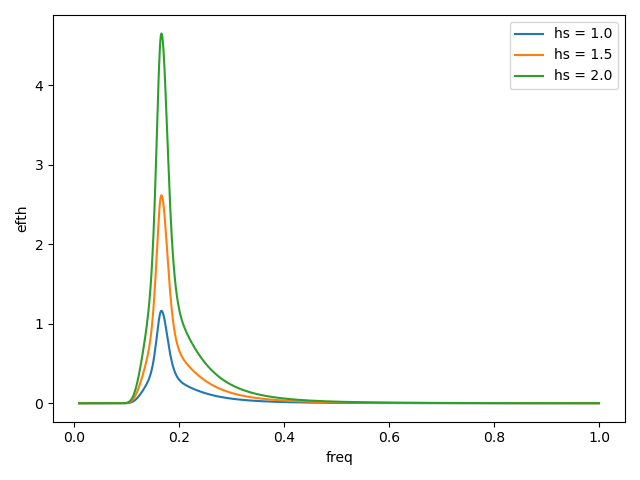
\includegraphics[width=0.7\textwidth]{Figures/figures/jonswap-wavespectra.png}
\end{center}
\subsubsection{Spreading (Étalement dans les fréquences)}
\label{sec:orgb3b3a3d}

Avec la fonction tirée de l'article de Cartwright (1963), on obtient un étalement directionnel de la forme (voir le \href{https://wavespectra.readthedocs.io/en/latest/construction.html\#cartwright-symmetrical-spread}{module en ligne}) : 
\begin{center}
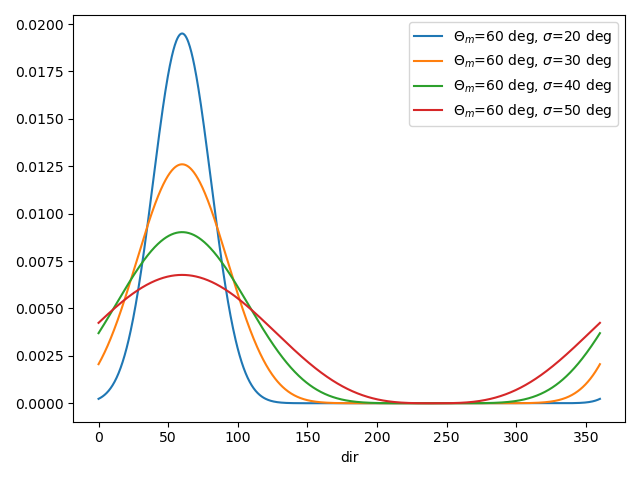
\includegraphics[width=0.7\textwidth]{Figures/figures/spreading.png}
\end{center}


Pour aucune raison, nous prendre un \(\sigma\) de 30 degrés. Grossièrement, la fonction d'étalement dans les fréquences devrait avoir la forme : 
\begin{equation}
   G(\theta,f)=F(s)cos^{2}\frac{1}{2}(\theta-\theta_{m}),
\end{equation}
et on a un spectre résultant  :

\begin{center}
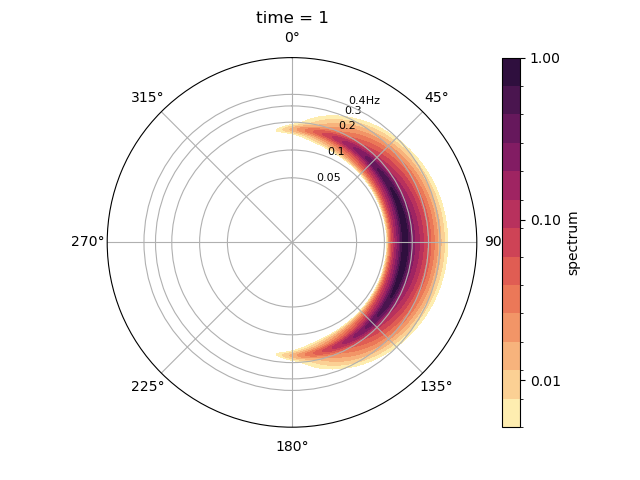
\includegraphics[width=0.7\textwidth]{Figures/figures/jonswap-wavespectra2.png}
\end{center}
\end{document}
